% Template per generare 

\documentclass[a4paper,11pt]{article}
\usepackage{lmodern}
\renewcommand*\familydefault{\sfdefault}
\usepackage{sfmath}
\usepackage[utf8]{inputenc}
\usepackage[T1]{fontenc}
\usepackage[italian]{babel}
\usepackage{indentfirst}
\usepackage{graphicx}
\usepackage{tikz}
\usepackage{listings}
\newcommand*\circled[1]{\tikz[baseline=(char.base)]{
		\node[shape=circle,draw,inner sep=2pt] (char) {#1};}}
\usepackage{enumitem}
% \usepackage[group-separator={\,}]{siunitx}
\usepackage[left=2cm, right=2cm, bottom=3cm]{geometry}
\frenchspacing

\newcommand{\num}[1]{#1}

% Macro varie...
\newcommand{\file}[1]{\texttt{#1}}
\renewcommand{\arraystretch}{1.3}
\newcommand{\esempioA}[2]{
\noindent\begin{minipage}{\textwidth}
\begin{tabular}{|p{7cm}|p{9cm}|}
	\hline
      \textbf{\file{input (da stdin)}} & \textbf{\file{output (su stdout)}}\\
	\hline
	\tt \small #1 &
	\tt \small #2 \\
	\hline
\end{tabular}
\end{minipage}
}
\newcommand{\esempioB}[2]{
\noindent\begin{minipage}{\textwidth}
\begin{tabular}{|p{9cm}|p{7cm}|}
	\hline
      \textbf{\file{input (da stdin)}} & \textbf{\file{output (su stdout)}}\\
	\hline
	\tt \small #1 &
	\tt \small #2 \\
	\hline
\end{tabular}
\end{minipage}
}

% Dati del task
\newcommand{\gara}{Esame Algoritmi 2019-06-25}
\newcommand{\nome}{Trascodifica di alberi ordinati: livello o discendenza?}
\newcommand{\nomebreve}{tree\_transcode\_level}

\begin{document}
% Intestazione
\noindent{\Large \gara}
\vspace{0.5cm}

\noindent{\Huge \textbf \nome~(\texttt{\nomebreve})}

% Descrizione del task
\section*{Descrizione del problema}

Un \emph{albero ordinato} consta di un \emph{nodo radice} e di una sequenza finita (eventualmente vuota) di \emph{figli} della radice, che sono a loro volta alberi ordinati. La figura offre due rappresentazioni dello stesso albero, nella prima su ogni nodo viene riportato il numero dei suoi discendenti (incluso il nodo stesso), nella seconda, su ogni nodo viene riportata la sua profondità, ossia la sua distanza dalla radice. Per convenzione, la radice viene disegnata in cima (cio\`e al contrario rispetto agli alberi veri).

\begin{figure}[h!]
  \centering
    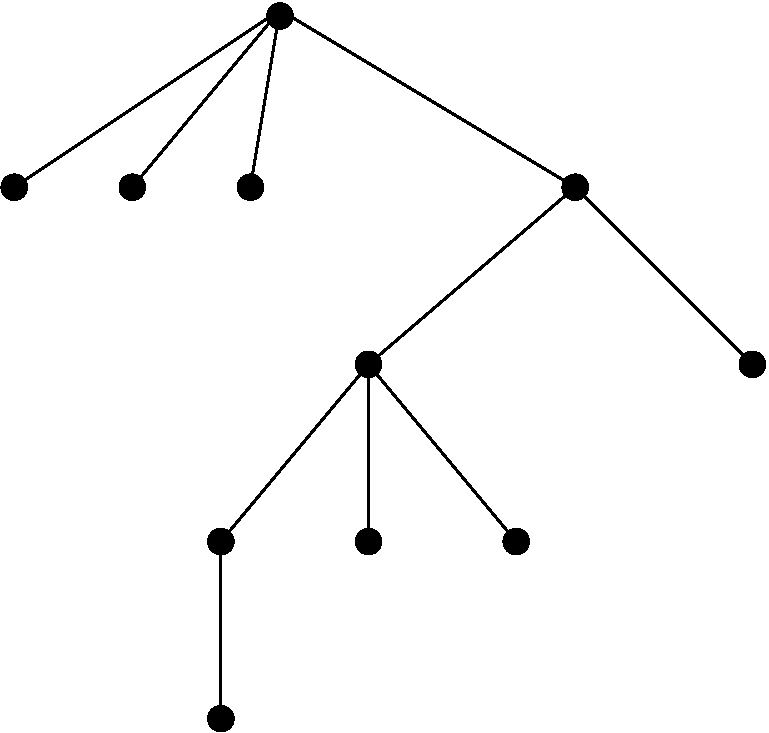
\includegraphics[scale=0.4]{figs/fig2.pdf}
      \quad \quad \quad \quad
    \includegraphics[scale=0.4]{figs/fig3.pdf}
    \caption{Un albero. A sinistra ogni nodo dichiara il numero di discendenti, a destra la profondità.}
\end{figure}

Proponiamo due possibili modi di codificare un albero come una sequenza di numeri naturali. Il primo numero della sequenza è~$1$ oppure~$2$
a seconda del sistema di codifica scelto.\\

\noindent
{\bf Codifica~1:}
Una sequenza di tanti numeri naturali quanti sono i nodi dell'albero. 
L'albero viene descritto dicendo quanti discendenti ha la radice (in questo caso 11) e poi descrivendo uno a uno, nell'ordine da sinistra a destra, i quattro sottoalberi. In questo modo, ad esempio, l'albero in figura sarebbe identificato dalla seguente sequenza:
\[
1\,\,\,11\,\,\,7\,\,\,1\,\,\,5\,\,\,1\,\,\,1\,\,\,2\,\,\,1\,\,\,1\,\,\,1\,\,\,1
\]	

Infatti, l'albero ha 11 nodi in tutto, ossia 11 sono i discendenti della radice (ogni nodo si considera discendente di se stesso), per cui il primo numero dopo lo specificatore di formato ($1$) \`e $11$. A questo $11$ segue poi subito la sequenza $7\,\,\,1\,\,\,5\,\,\,1\,\,\,1\,\,\,2\,\,\,1$, che \`e la descrizione del primo sottoalbero, mentre gli ultimi tre sottoalberi sono ciascuno descritti da $1$ (dato che non hanno alcun figlio).

\noindent
{\bf Codifica~2:}
Quì la sequenza è lunga il doppio in quanto ogni nodo parla due volte:
sia in apertura che in chiusura del sottoalbero di cui egli è radice.
In entrambe le occasioni, il nodo dice la propria profondità entro l'albero, ossia il numero di archi nell'unico cammino che lo collega alla radice.
A parte queste differenze, l'ordine in cui ogni sottoalbero viene aperto è lo stesso che per la Codifica~1. 
Nella seconda codifica la sequenza generata dall'albero in figura è la seguente:
\[
2\,\,\,0\,\,\,1\,\,\,2\,\,\,2\,\,\,2\,\,\,3\,\,\,3\,\,\,3\,\,\,3\,\,\,3\,\,\,4\,\,\,4\,\,\,3\,\,\,2\,\,\,1\,\,\,1\,\,\,1\,\,\,1\,\,\,1\,\,\,1\,\,\,1\,\,\,0
\]	



% Input
\section*{Dati di input}

L'input deve avvenire da stdin, da dove il vostro programma legge una sola riga contenente la codifica di un albero offerta secondo il primo o secondo formato.

% Output
\section*{Dati di output}

L'output deve avvenire su stdout, dove il vostro programma deve restituire una sola riga:
la codifica dello stesso albero nell'altro formato.

% Esempi
\section*{Esempio di input/output}
\esempioA{
1 11 7 1 5 1 1 2 1 1 1 1
}{
2 0 1 2 2 2 3 3 3 3 3 4 4 3 2 1 1 1 1 1 1 1 0
}


\section*{Esempio di input/output}
\esempioB{
2 0 1 2 2 2 3 3 3 3 3 4 4 3 2 1 1 1 1 1 1 1 0
}{
1 11 7 1 5 1 1 2 1 1 1 1
}

% Assunzioni
\section*{Assunzioni}
\begin{itemize}[nolistsep, noitemsep]
\item dove $n$ \`e il numero di nodi dell'albero,
      vale sempre che $1 \le n \le 1\,000\,000 $;
\item tempo limite: un secondo.
\end{itemize}

% Subtasks
\section*{Subtask}
Un totale di $100$ punti \`e ripartito su $2*5=10$ subtask.
Il subtask coi casi di esempio non dà punti.
\begin{itemize}
\item \textbf{Subtask 1 [0 punti]:} l'esempio del testo.
\item \textbf{Subtask 2+x [10 punti]:} ogni nodo ha massimo un figlio.
\item \textbf{Subtask 3+x [10 punti]:} ogni nodo ha massimo due figli.
\item \textbf{Subtask 4+x [10 punti]:} $N \le 10$.
\item \textbf{Subtask 5+x [10 punti]:} $N \le 1000$.
\item \textbf{Subtask 6+x [10 punti]:} $N \le 1\,000\,000$.
\end{itemize}
Come interpretare $x$: alcune istanze ($x=0$) chiedono di passare dalla prima alla seconda codifica,
altre ($x=5$) chiedono di passare dalla seconda alla prima codifica.


\end{document}
